\section{Background}
Methods, literature, related work (perhaps as a separate subsection)
Description of GCP, K8s, infrastructure background

\subsection{Ground Truth}
\subsubsection{Open PageRank}
\label{OpenPageRank}
\textit{Open PageRank} \cite{OpenPageRank} is an initiative, which has the goal to enable webmasters to determine the pagerank for their domains and easily compare with other domains. The initiative was constituted after Google had shut down the \textit{PageRank}-toolbar, leaving a void in the industry. The Open PageRank initiative provides freely available data that was built on top of \textit{Common Crawl} \cite{CommonCrawl}, which provides high quality crawl data of webpages since 2013.

Open PageRank uses the number of backlinks of a domain found in \textit{Common Crawl} to calculate the pagerank. The greater the number of links, different domains use to refer to the given domain, the better the pagerank of the given domain according to Open PageRank.

\subsection{Kubernetes \cite{SAPTerraformSamed}}
Kubernetes is an open source container orchestration solution that was originally designed by \textit{Google} in 2014. It aims to provide a platform where containers and containerized applications can be deployed, scaled and managed \cite{Wikik8s}. K8s orchestrates computing, networking, and storage infrastructure on behalf of user workloads. This means that applications are automatically scaled depending on incoming workload.

K8s is much of the simplicity of Platform as a Service with the flexibility of Infrastructure as a Service \cite{k8s}. K8s offers platform abstraction at container level. From this follows that developers are responsible for building their own application containers rather than only the application itself. This is rewarded with more freedom in application development, but punished with less productivity.

\subsubsection{Kubernetes Components and Concepts}
The most known container runtime in industry is \textit{Docker}. Container runtimes are responsible for serving the communication to the OS and the container environment, where application can be configured and run.
\begin{figure}
	\centering
	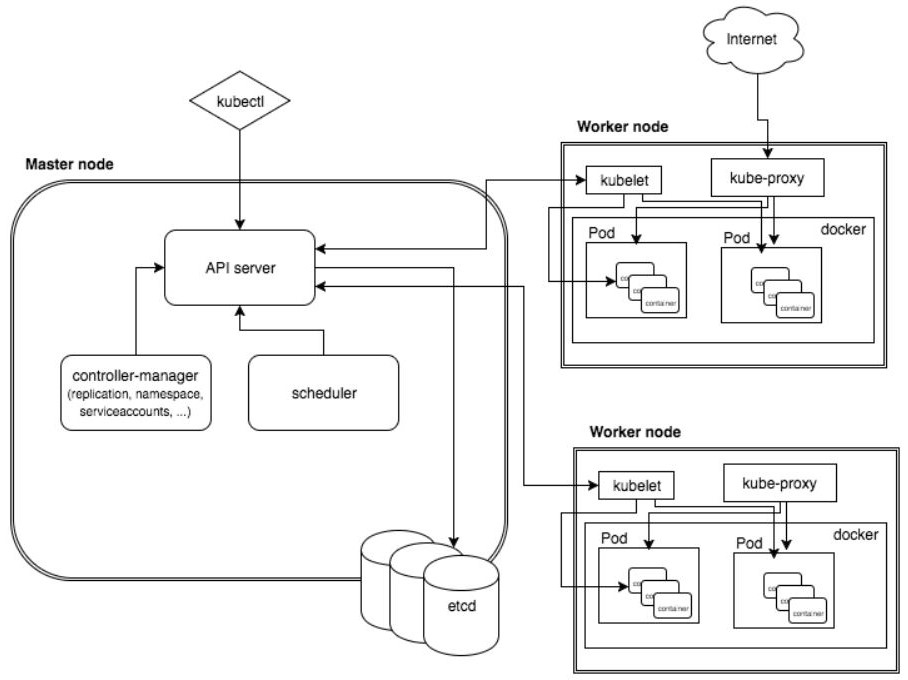
\includegraphics[width=0.8\textwidth]{resources/k8s_architecture}
	\caption{Architecture Diagram of K8s \cite{K8sArch}}
	\label{k8s_architecture}
\end{figure}
K8s consist of three main components \textit{kubectl}, \textit{master node} and the \textit{worker nodes}. While kubectl represents the client interface to communicate with the master node by sending request against the API server. The master node represents the administrative entrypoint and is responsible for managing the whole K8s cluster \cite{K8sArch}. It consists of the \textit{API server}, \textit{etcd storage}, \textit{scheduler} and \textit{controller manager}:

\begin{itemize}
	\item \textit{API server} represents the entry points for all incoming REST commands. It processes them and executes it according to their business logic.
	\item \textit{etcd storage} is a simple key-value store, where information about the \textit{pods} and the cluster is saved.
	\item \textit{scheduler} is responsible for container distribution among the worker nodes by using information about the worker nodes. 
	\item \textit{controller-manager} consists of several controllers such as the replication controller, which is responsible for monitoring pods and recreating crashed pods.
\end{itemize}
Beside the master node a K8s cluster consists of one or more worker nodes, which are controller by the controllers of the master node. Each worker node consists of \textit{kubelet}, \textit{kubeproxy} and \textit{pods}:

\begin{itemize}
	\item \textit{kubelet} communicates with the API server for ensuring that the requested containers are up and running.
	\item \textit{kube-proxy} acts as a proxy and load balancer on the worker node. It is responsible for the communication with the outer world.
	\item \textit{pods} is the smallest unit in K8s. It encapsulates one or many other containers in same shared context, which means that containers within the same pods share the same ip, storage and memory.
\end{itemize}